%%% LaTeX Template: Curriculum Vitae
%%%
%%% Source: http://www.howtotex.com/
%%% Feel free to distribute this template, but please keep the referal to HowToTeX.com.
%%% Date: July 2011

%%% ------------------------------------------------------------
%%% BEGIN PREAMBLE
%%% ------------------------------------------------------------
\documentclass[paper=a4,fontsize=11pt]{scrartcl}	 			% KOMA-article class
							
%\usepackage[english]{babel}								% English language/hyphenation
%\usepackage[protrusion=true,expansion=true]{microtype}		% Better typography
\usepackage{hyperref}
\usepackage{amsmath,amsfonts,amsthm}					% Math packages
\usepackage[pdftex]{graphicx}								% Enable pdflatex
\usepackage[svgnames]{xcolor}							% Colors by their 'svgnames'
\usepackage{geometry}
	\textheight=700px									% Saving trees ;-) 
\usepackage{url}										% Clickable URL's
\usepackage{wrapfig}									% Wrap text along figures

\frenchspacing									% Better looking spacings after periods
\pagestyle{empty}								% No pagenumbers/headers/footers
%\usepackage{bbding}									% Symbols

%%% Custom sectioning (sectsty package)
%%% ------------------------------------------------------------
\usepackage{sectsty}							% Custom sectioning (see below)

\sectionfont{%									% Change font of \section command
	\usefont{OT1}{phv}{b}{n}%					% bch-b-n: CharterBT-Bold font
	\sectionrule{0pt}{0pt}{-5pt}{3pt}
	}

%%% Macros
%%% ------------------------------------------------------------
\newlength{\spacebox}
\settowidth{\spacebox}{8888888888}				% Box to align text
\newcommand{\sepspace}{\vspace*{1em}}			% Vertical space macro

\newcommand{\MyName}[1]{
		\Huge \usefont{OT1}{phv}{b}{n} \hfill #1 		% Name
		\par \normalsize \normalfont}
		
\newcommand{\MySlogan}[1]{
		\large \usefont{OT1}{phv}{m}{n}\hfill \textit{#1} % Slogan (optional)
		\par \normalsize \normalfont}

\newcommand{\NewPart}[1]{\section*{\uppercase{#1}}}

\newcommand{\PersonalEntry}[2]{
		\noindent\hangindent=2em\hangafter=0 		% Indentation
		\parbox{\spacebox}{						% Box to align text
		\textit{#1}}								% Entry name (birth, address, etc.)
		\hspace{1.5em} #2 \par}					% Entry value

\newcommand{\SkillsEntry}[2]{						% Same as \PersonalEntry
		\noindent\hangindent=2em\hangafter=0 		% Indentation
		\parbox{\spacebox}{						% Box to align text
		\textit{#1}}								% Entry name (birth, address, etc.)
		\hspace{1.5em} #2 \par}					% Entry value	
		
\newcommand{\EducationEntry}[4]{
		\noindent \textbf{#1} \hfill 					% Study
		\colorbox{Black}{%
			\parbox{8em}{%
			\hfill\color{White}#2}} \par				% Duration
		\noindent \textit{#3} \par					% School
		\noindent\hangindent=2em\hangafter=0 \small #4 	% Description
		\normalsize \par}

\newcommand{\WorkEntry}[4]{						% Same as \EducationEntry
		\noindent \textbf{#1} \hfill 					% Jobname
		\colorbox{Black}{\color{White}#2} \par		% Duration
		\noindent \textit{#3} \par					% Company
		\noindent\hangindent=2em\hangafter=0 \small #4 	% Description
		\normalsize \par}
		
\newcommand{\BibEntry}[2]{
		\noindent \textbf{#1} \hfill \par					% Study
		\noindent\hangindent=2em\hangafter=0 \small #2 	% Description
		\normalsize \par}
		
		



%%% ------------------------------------------------------------
%%% BEGIN DOCUMENT
%%% ------------------------------------------------------------
\begin{document}
\begin{wrapfigure}{l}{0.5\textwidth}
	\vspace*{-4em}
		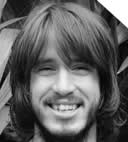
\includegraphics[width=0.2\textwidth]{Doug-Kelley.jpg}
\end{wrapfigure}

\MyName{Douglas Kelley}
\MySlogan{Curriculum Vitae}

\sepspace

%%% Personal details
%%% ------------------------------------------------------------
\NewPart{Personal details}{}

\PersonalEntry{Birth}{6th August, 1984} 
\PersonalEntry{Address}{6/1 Tasman Pl. Macquarie Park, NSW, Australia, 2113}
\PersonalEntry{Phone}{+61 (0) 468790426}
\PersonalEntry{Mail}{\url{douglas.kelley@mq.edu.au}}

%%% Education
%%% ------------------------------------------------------------
\NewPart{Education}{} 

\EducationEntry{\href{http://bcd.mq.edu.au/?page_id=171}{PhD Ecology}}{2010-Jan 2014}{\href{http://bio.mq.edu.au/}{Biological Scicence, Macquarie University}}
  {\textbf{\href{http://bcd.mq.edu.au/?p=361}{Modelling Australian fire regimes under furture climate change.}} Benchmarking and developing the LPX Dynamic Global Vegetation Model (DGVM) fire-vegetation interacting and applying it for simlating 21st century fire and vegetatation in Australia}
\sepspace

\EducationEntry{\href{http://www.bristol.ac.uk/cabot/postgrad/msc-ccsp.html}
             {MSc. Earth System Science}}{2007-2008}{\href{http://www.bristol.ac.uk/earthsciences/}{Earth Sciences, Bristol University}}
  {\textbf{Main dissitation: Statistical modelling of global fire regimes.} Climate change science and policy; Earth system modeling; Remote sensing of the environment and GIS}
\sepspace

\EducationEntry{\href{http://www2.warwick.ac.uk/study/undergraduate/courses/f300}{BSc. Physics}}{2002-2007}{\href{http://www2.warwick.ac.uk/fac/sci/physics/}{Physics, University of Wariwck}}
  {Main dissitation: Modelling atmospheric effects on starlight.}
  
  
\NewPart{Publications}

\BibEntry{In Refereed Journals}{\href{http://onlinelibrary.wiley.com/doi/10.1002/jgrg.20118/abstract}{Kaminski, T., Knorr, W., Sch, G., Scholze, M., Rayner, P. J., Zaehle, S., Blessing, S., Dorigo, W., Gayler, V., Giering, R., Gobron, N., Grant, J. P., Houweling, S., Kato, T., Kattge, J., \textbf{Kelley, D. I.}, Kemp, S., Koffi, E. N., Mathieu, P. P., Pinty, B., Reick, C. H., Vossbeck, M., Widmann, H. and Ziehn, T.: The BETHY / JSBACH Carbon Cycle Data Assimilation System : experiences and challenges, Journal of Geophysical Research, available online, 2013.}}


\BibEntry{} {\href{http://www.biogeosciences.net/10/3313/2013/bg-10-3313-2013.html}{\textbf{Kelley, D. I.}, Prentice, I. C., Harrison, S. P., Wang, H., Simard, M., Fisher, J. B. and Willis, K. O.: A comprehensive benchmarking system for evaluating global vegetation models, Biogeosciences, 10(5), 3313-3340, 2013.}}


\BibEntry{} {\href{http://www.nature.com/ngeo/journal/v5/n1/full/ngeo1324.html}{Ciais, P., Tagliabue, a., Cuntz, M., Bopp, L., Scholze, M., Hoffmann, G., Lourantou, a., Harrison, S. P., Prentice, I. C., \textbf{Kelley, D. I.}, Koven, C. and Piao, S. L.: Large inert carbon pool in the terrestrial biosphere during the Last Glacial Maximum, Nature Geoscience, 5(1), 74-79, 2012.}}


\BibEntry{} {\href{http://onlinelibrary.wiley.com/doi/10.1029/2010GB003906/abstract}{Prentice, I. C., \textbf{Kelley, D. I.}, Foster, P. N., Friedlingstein, P., Harrison, S. P. and Bartlein, P. J.: Modeling fire and the terrestrial carbon balance, Global Biogeochemical Cycles, 25(3), 1-13, 2011.}}
\sepspace
\pagebreak

\BibEntry{Submitted} {Harrison, S. P., \textbf{Kelley, D. I.}, Wang, H., Herbert, A., Li, G., Bradstock, R., Fontaine, J., Enright, N., Murphy, B. P., Penman, T. and Russell-Smith, J.: Patterns in fire-response trait abundances in Australia using a new database of plot-level measurements for fire model evaluation., Global Ecology and Biogeography.}

\BibEntry{} {\textbf{Kelley, D. I.}, Harrison, S. P. and Prentice, I. C.: Improved simulation of fire-vegetation interactions in the Land surface Processes and eXchanges Dynamic Global Vegetation Model (LPX-Mv1), Geoscientific Model Development Discussions.}
\sepspace

\BibEntry{In prep.} {\textbf{Kelley, D. I.}, Harrison, S. P.: Impact of re-sprouting on future forest surival and carbon stocks in fire-prone ecosystems.}

\BibEntry{} {Zeppel, M., Adams, H., West, A., \textbf{Kelley, D. I.}, Medlyn, B., Fensham, R., Dawson, T., Tissue, D. and Harrison, S.: Drought-induced mortality within resprouters.}

\NewPart{Awards}
\EducationEntry{\href{http://www.hdr.mq.edu.au/information_for/current_candidates/financial_support}{Post Graduate Reasearch Fund (PGRF)}}{2013} {Macquarie University - Competetive award to enhance postgraduate research experience}{Funding presentation of vegegation model development and enhanced future projection of terrestial carbon stocks under climate change at AGU fall conference}
\sepspace
\EducationEntry{Biology postgrad conference best presentataion}{2011} {Biological Sciences,Macquarie University}{Best presentation out of the departments 78 postgraduate students at the annual post-graduate conference. Awarded from presentation on vegetation model benchmarking system}
\sepspace
\EducationEntry{Intenational Macquarie University Research \\ Excellence Scholarships (iMQRES)}{2010-2014} {Macquarie University postgraduate award}{For completion of PhD. thesis}


%%% Work experience
%%% ------------------------------------------------------------
\NewPart{Relevant Work experience}{}

\EducationEntry{Reasearch Assistant}{2008-2010}{University of Bristol, Full-time}
  {Job description goes here. To maintain a stylish look, try to fill this description with a few lines of text. Do the same for the other entries in this section.}
\sepspace

\EducationEntry{Earth System Science Summer School co-ordinator}{2008}{Department of Earth Science, Bristol University, Part-time}{Publicty, lecture and seminar timetabling, finding and organising guest lectures, general admin}
\sepspace 

\EducationEntry{Widening Participation }{2008}{Widening Participation Office, Bristol University, Part-time}{orking with students in primary and secondary education to encourage university attendance from low socio-economic backgrounds. Help organize \& run University open days and campus tours. In-school presentations and career evening.}

\NewPart{Relevant Extra-Circular activity}{}
\EducationEntry{Committee member responsible for Web-design,\\ Communications, and social runners}{2011-present}{Epping and District Athletics Clubs}
  {Website development (www.eppingdac.com), newlsetter (www.eppingdac.com.au/newsletter) and e-publicty for local communittee running and athletics club}
\sepspace  

\EducationEntry{Student Union involvment}{2002-2008}{University and Warick/Bristol University}
  {Sabatical year sitting on board of directors responsible for student advice and welfare department, 3 years as charity trustee and 6 years on student council resposble for Science Faculty representation. Committe posts on various student run sports clubs and societies including People and Planet, Student TV station, Student Support Groups, and running club}
\sepspace  

\BibEntry{Digital Phtography and art}{www.}




\


%%% Skills
%%% ------------------------------------------------------------
\NewPart{Skills}{}

%\SkillsEntry{Programming Code}{Fortran}
%\SkillsEntry{}{C}
%\SkillsEntry{}{C++} 


\SkillsEntry{Programming}{Fortran, \textsc{C++}, C, Shell, R, \textsc{Python}, \textsc{Matlab}, VB.}
\SkillsEntry{Languages}{\textsc{Git} and svn version control (see www.bit...)} 
\vspace{1cm}
\SkillsEntry{Publishing}{html/css/\textsc{php}, \LaTeX, GIMP, Scribus, \textsc{Photoshop/Illustrator},}
\SkillsEntry{Languages/}{plus standard office/open office software}
\SkillsEntry{Software}

%%% References
%%% ------------------------------------------------------------
\NewPart{References}{}
Available upon request


%\nocite{*} 
%\bibliographystyle{plain}
%\renewcommand{\bibname}{References}
%\bibliography{my_papers.bib}

\end{document}